\documentclass[12pt, titlepage]{article}
\usepackage[margin=1in]{geometry}
\usepackage{graphicx}
\usepackage{float}

%\usepackage{hyperref}

\title{\Huge Feedback Controls Fall Final Design Report \\ \normalsize{EGEE 4810 - Senior Design}}
\author{by \\ \Large TEAM WINGFEATHER \\ Aydan Vissing \\ Brady Schick \\ Gabriel Southwell \\ Simon Ross}
\date{\footnotesize{Due} \\ \normalsize{December 12, 2025}}


%\setlength{\topmargin}{-.25in}
%\setlength{\oddsidemargin}{.25in}
%\setlength{\evensidemargin}{.25in}
%\setlength{\textwidth}{6.0in}
%\setlength{\textheight}{9.0in}
%\renewcommand{\baselinestretch}{1.4}
%\usepackage{indentfirst} %Maybe keep this maybe not

\begin{document}
\maketitle

%FIXME remove comments

%FIXME improve abstract
\begin{abstract}
This project report summarizes the progress to date on project Wingfeather, intended to reimagine the Feedback Controls Laboratory experience at Cedarville University. The main goals of this project are to make the lab experience more engaging and relevant for students, simpler to work with, more reliable than previous solutions, and more cost-effective. To achieve these ends, progress has been made towards a cheap drone platform that is capable of communicating fundamental feedback controls concepts along with a simple software user interface. Up to this point, hardware has been developed for the fabrication of a printed circuit board with the necessary components. This board has been acquired, and sensor communication code is in the integration phase. A mathematical model has been created to describe the drone dynamics, and will also be integrated soon. As the project continues to mature, the rest of the selected components will be integrated onto a custom 3D-printed frame and the testing phase will begin. Ultimately, this project is on track to be completed by the end of next semester. The current status shows promise to transform the way students view Feedback Controls lab, relating classwork to concepts they are familiar with and making lab time more enjoyable.


\end{abstract}

\newpage
\tableofcontents
%\listoffigures
%\listoftables

\newpage
\section{Definition Statement}

This project seeks to redefine the Cedarville Feedback Controls Laboratory experience by designing a quadcopter drone to use as an entertaining platform to teach classroom concepts. 

\section{Introduction \& Background}

The current lab experience for EGME-4660 uses the Feedback Analogue Unit 33-110 and the Feedback Mechanical Unit 33-100. Although the labs using the equipment do cover the desired content, they are often tedious and perhaps confusing to new users, especially users unfamiliar with Feedback Controls concepts. The user interface to conduct the experiments is a circuit board with nodes and banana plug cords. The user can connect these nodes to create feedback circuits whose effect is then shown using the mechanical unit. As mentioned, understanding what is happening between the units (and even in the electrical circuits) can be challenging for students. This causes the applications of the class material to  seem boring and irrelevant, especially for mechanical engineering students who may not have extensive electronics background. In addition, the equipment is old and fragile - adjusting the power supply or wiring the power incorrectly can result in damage to the equipment, often requiring parts to be replaced. Since the equipment is out of production and thus quite expensive, the current repair method has been de-soldering and soldering components by hand. We plan to improve the lab experience by replacing the current equipment with cheap and robust drones that can be reprogrammed for the purposes of the lab with a user-friendly interface. In this way, the instructor can choose the complexity of the tasks given to students for the lab.

\section{Objectives}
\subsection{Marketing Requirements}

The following requirements define the end user experience as desired by the customer:
  \begin{itemize}
    \item The final product must focus on autonomous actuation and control.
    \item The laboratory experience must include the ability to implement a PID control design.
    \item The final product must be able to physically and graphically display a step response.
    \item The students must have the opportunity to measure a Bode plot in real life.
    \item The laboratory experience must include the ability to see and correct the effects of physical and observable disturbances and noise.
    \item The final product should showcase the results of controllers physically in real life and not just with numbers and data.
    \item The final product must have the ability to log data to a neutral format independent of real time visualizations.
    \item The software solution must include a widget to generate understandable plots of the data.
    \item The final laboratory experience must include the capability to perform a tracking experiment.
    \item The laboratory experience must take relevant safety precautions.
    \item The final platform must be able to implement open loop control and log this response. 
  \end{itemize}
\subsection{Engineering Requirements}
\subsubsection{Hardware Requirements}
\begin{itemize}
  \item Hard Requirements:
  \begin{itemize}
    \item Microcontroller
    \item 4 motors
    \item Battery power supply
    \item PCB to interconnect components
    \item Bladeguards for safety
    \item Positional and tracking sensors
  \end{itemize}
  \item Soft Requirements:
  \begin{itemize}
    \item Sturdy frame
    \item Conviently swappable and rechargable batteries
  \end{itemize}
\end{itemize}
\subsubsection{Software Requirements}
\begin{itemize}
  \item Hard Requirements:
  \begin{itemize}
    \item PID controller logic so drone can fly
    \item Controller logic for open loop capabilities
    \item Memory for data collection
    \item User-friendly interface for programming
    \item Method to input step functions and sinusoidal functions
  \end{itemize}
  \item Soft Requirements:
  \begin{itemize}
    \item Wireless communication
    \item Intuitive GUI
    \item Software to plot collected data
  \end{itemize}
\end{itemize}
\subsection{Constraints}
\begin{itemize}
  \item The laboratory experiments must be able to be conducted in ENS 145 at Cedarville University.
  \item The total cost of design, test, and evaluation must not exceed \$600.
  \item The final laboratory experience must not endanger the safety of the students.
  \item The final laboratory solution must not not destroy Cedarville property.
  \item The final laboratory experience must not use MATLAB.
\end{itemize}

\section{Engineering Design}
The sections below outline major design decisions that have been made over the past semester in the areas of software, hardware, and controls. Also included are some future plans for development in these areas.

\subsection{Hardware}
\begin{enumerate}

\item Custom PCB
\begin{itemize}
\item Successfully designed and ordered the first version of the PCB
\item PCB provides support to drone frame, but the frame is not comprised by it
\end{itemize}

\item Microcontroller
\begin{itemize}
\item Model selected: ESP32\_WROOM\_32N8 
\item Fast microcontroller with plenty of RAM
\item 2 cores for supporting sensor I/O, motors, and multiple PID loops
\item Has an integrated antenna for wireless data transfer - see software section below
\item Buttons included to reset microcontroller and start script
\end{itemize}

\item Inertial Measurement Unit (IMU)
\begin{itemize}
\item Model selected: MPU-6050
\item Accurately senses rotation in 3 axes for calculating error
\item Includes both MEMS gyroscope and accelerometer for 6 axis measurements
\item Currently successfully receiving IMU data both wired and wirelessly.
\end{itemize}

\item Buzzer
\begin{itemize}
\item Model selected: FUET-8540-3.6V
\item Added buzzer to design for auditory feedback
\end{itemize}

\item LEDs
\begin{itemize}
\item Added 3 LED array for visual feedback
\end{itemize}

\item Connector
\begin{itemize}
\item Decided to use USB-C for connection to lab computers
\end{itemize}

\item Power Regulator
\begin{itemize}
\item Model selected: TPS63070RNMR
\item Decided to use buck/boost converter instead of a standard power regulator
\item Input range of 2-16V
\item Output voltage is 3.3V
\end{itemize}

\item Sensors
\begin{itemize}
\item Model selected: VL53L1
\item Mounting these sensors on the main PCB proved to be expensive and complicated, so we decided to use smaller boards to be soldered on to the main board
\item Range of 4 m, meaning we are able to see both the roof and floor at the same time. This will help with decision logic if the drone flies over an object
\item Decided to mount sensors on the top and bottom of the drone and 3 on the sides. This allows for accurate altitude measurements and ranging from walls. Additionally, by placing 2 sensors on one side of the drone, a heading may be calculated
\item Currently successfully receiving sensor data both wired and wirelessly.
\end{itemize}

\item Motors and Motor Controllers
\begin{itemize}
\item 720 coreless DC motors selected
\item Since the motors are brushed and only need to turn in one direction, MOSFETs are used instead of a full motor controller IC
\end{itemize}

\item Special Circuitry
\begin{itemize}
\item Diode circuit added to allow powering of the circuit by a battery, connected computer, or even both (without damage)
\item ESD and reverse current protection circuits included
\item Auto reset logic circuit included so the microcontroller enters the bootloader properly when a computer is connected
\end{itemize}

\item Battery
\begin{itemize}
\item 2 battery connector options included on the PCB - user may select which connector they are using and solder it on
\item The power converter accepts a large range of battery voltages, allowing for the use of 1, 2, or 3 cell LiPo batteries
\item Battery choices are flexible (helpful, considering needs may change). This way we can increase the voltage to the motors if needed.
\item Planning to need some sort of charging array for the students to each receive multiple batteries per lab session
\end{itemize}

\item Frame
\begin{itemize}
\item Cheap, light, strong 3D printed frame created that successfully holds the motors, battery, and printed circuit board
\item Adjustments being made to the print integrity and sensor placement on the frame
\end{itemize}

\end{enumerate}

\subsection{Software}
\begin{enumerate}
	\item Drone Firmware
	\begin{itemize}
		\item FreeRTOS
		\begin{itemize}
			\item Real Time Operating System that is built and optimized for microcontrollers. An RTOS is a system for switching between many processes. This will allow the system to constantly check sensor, log data, and run the flight logic all at the same time.
		\end{itemize}
		\item Wireless Telemetry
		\begin{itemize}
			\item Drones act as WiFI access points and send out UDP packets to all devices connected to the AP
			\item Computers can connect to the AP and receive the packets with a simple listener program that converts the packets into CSV
		\end{itemize}
		\item Non-volatile telemetry
		\begin{itemize}
			\item Lines of CSV from the sensors are written to a RAM buffer. When the buffer is full, it gets flushed to a partition on the flash that was made using LittleFS. This is done to save write cycles on the flash since cheap flash storage has limited writes. The CSV can be retrieved by rebooting the drone, plugging it into a laptop, and running a flash dump script that outputs the full CSV.
		\end{itemize}
		\item Fight Configuration/Controls
		\begin{itemize}
			\item The drone will get its flight configuration and flight script from a script file that will be loaded into the LittleFS by the desktop app. 
		\end{itemize}
		\item PID Flight Loop
		\begin{itemize}
			\item Most of this part will be taken from an existing drone project like ESP-Drone or BetaFlight
		\end{itemize}
		\item I$^2$C Sensor Communication
		\begin{itemize}
			\item Successfully implemented sensor readdressing code. This means that each sensor's data can be individually recorded. Communication with the IMU and the time of flight sensors has been established simultaneously.
		\end{itemize}
	\end{itemize}
	\item Desktop Application
	\begin{itemize}
		\item Design
		\begin{itemize}
			\item The GUI will be made with QTDesigner which is a cross-platform WYSIWYG GUI editor
			\item The back-end will be written in Python since it is supported by QTDesigner and all the desktop scripts that have been written are already in Python 
		\end{itemize}
		\item Scripting
		\begin{itemize}
			\item The app will have some method for creating configuration and flight script files. These files will be uploaded to the drone using ESPTool
		\end{itemize}
		\item Telemetry
		\begin{itemize}
			\item Will contain methods for receiving telemetry both wirelessly and from the LittleFS partition. 
			\item Might also include some type of data visualization system
		\end{itemize}
	\end{itemize}
\end{enumerate}

\subsection{Controls}
\begin{enumerate}
		\item Non-Linear Model
		\begin{figure}[htbp]
    			\centering
    			\includegraphics[width=0.9\textwidth]{ControlsFlowchart}
    			\caption{Control Loop for Quad-copter Flight}
    			\label{fig:myimage}
		\end{figure}
		\begin{itemize}
			\item Fully defines how the drone will be controlled in software using PID controllers.
			\item PID controllers were used for their simplicity and their widespread use in controls fields
		\end{itemize}
		\item Linear Model
		\begin{itemize}
			\item Allows for mapping of poles of the control system
			\item This helps the tuning process to avoid producing an unstable system
		\end{itemize}
		\item Simulation
		\begin{itemize}
			\item Quad-copter dynamics and controls simulated using MATLAB
			\item Allows for verification of quad-copter dynamics and controls
			\item Provides functionality for an initial start to the tuning process 
		\end{itemize}
\end{enumerate}

\section{Project Schedule}
Figure 2 below shows an up-to-date version of our project schedule. Dates over semester 1 are the events that have taken place while the second semester remains notional. Up to this point, the project has remained incredibly close to the proposed schedule, as can be seen by comparing this report with our proposal. 

\begin{figure}[H]
  \centering
  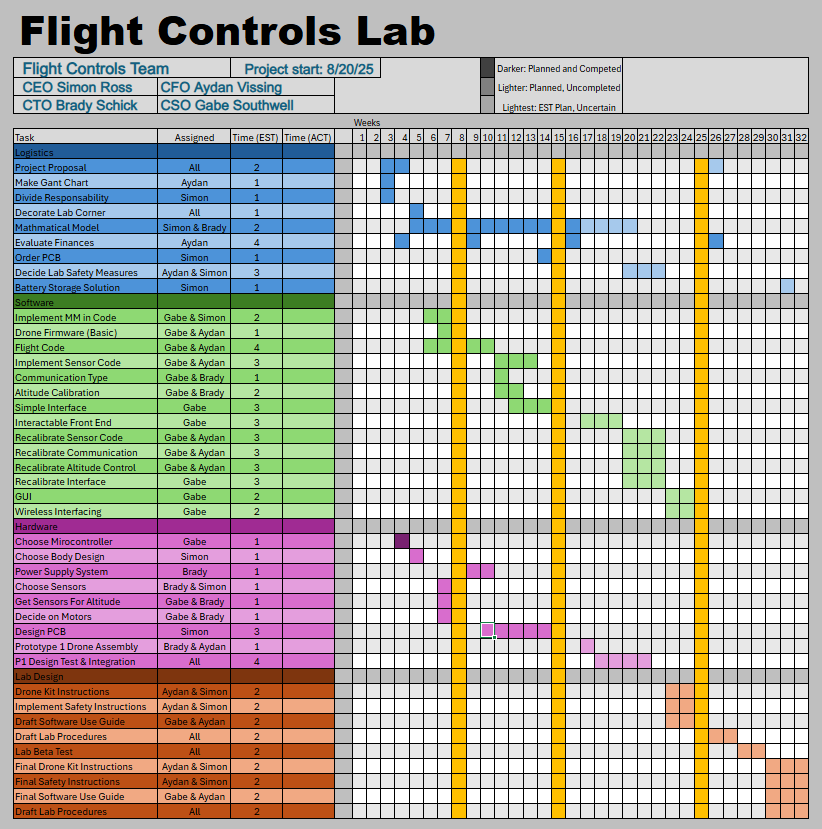
\includegraphics[width=5.7in]{../gantt/gantt_2_0.png}
  \caption{Project Gantt Chart Schedule}
  \label{fig:gantt}
\end{figure}


\section{Project Summary}

\subsection{Current Progress}

As of now, we have a fully designed PCB, an almost fully designed drone frame, and the majority of the parts needed to assemble the quadcopter. A lot of the work has also been done in setting up the drone firmware and designing the flight controls. Moving forward, we plan to assemble the drone and finish up the firmware and controls. Then, we will be able to move on to controller tuning, lab design, and setting up the desktop application.

\subsection{Milestones}

\subsubsection[October 3, 2025]{Milestone 1: October 3, 2025} By this date, we selected and ordered all of the components needed to construct a prototype drone (using perfboard instead of a PCB) by this date. Additionally, this time was spent researching open source software options for working with the selected components. 

\subsubsection[November 14, 2025]{Milestone 2: November 14, 2025} This milestone was modified part of the way into the semester as recommended by Dr. Kohl and Dr. Fredette - instead of having a hardware prototype, we instead produced a fully designed PCB and ordered it. This way we can use winter break to debug the PCB for the beginning of next semester.

\subsection{Budget}
The budget below describes how we intend to use funds in constructing a prototype. Under this paradigm, we will be far under our proposed budget of \$600. However, this budget does not account for mistakes in prototyping and drastic changes to the program. This budget is up to date with what we have spent on each component so far.

\begin{table}[H]
\centering
\caption{Unit Budget for Feedback Controls Lab Prototype}
\label{tab:budget}
\begin{tabular}{||c|c|c|c||}
\hline 
\hline
\textbf{Component/Expense} & \textbf{Price} & \textbf{Order Date} & \textbf{Comments} \\ 
\hline 
Prototype Microcontroller & \$0 & N/A & Dr. Kohl gave us one to borrow \\
\hline 
Time of Flight Sensors & \$37 & 19-Sep & 2 Orginal + Additional 10 \\
\hline 
Motors & \$10 & 19-Sep & 4 motors \\ 
\hline 
Body & \$0 & N/A & 3D printed \\ 
\hline 
Props & \$7 & 19-Sep & As many props as we can get \\ 
\hline 
Battery & \$15 & 19-Sep & $\sim$500mAh Lithium \\ 
\hline 
PCB(s) & \$67 & 15-Nov & 3 boards for redundancy \\ 
\hline 
\textbf{Total Cost} & \textbf{\$134} &  &  \\ 
\hline 
\hline
\end{tabular} 
\end{table}


\end{document}
